\documentclass[12pt, letterpaper]{article}
\usepackage{graphicx} % Required for inserting images
\usepackage{hyperref}
\usepackage{listings}
\usepackage{amssymb}
\usepackage{amsmath}
\usepackage[english]{babel}
\usepackage{nicefrac, xfrac}
\usepackage{mathtools}
\newcommand{\acc}{\\\hphantom{}\\}
\usepackage[table,xcdraw]{xcolor}
\definecolor{light-gray}{gray}{0.95}
\newcommand{\code}[1]{\colorbox{light-gray}{\texttt{#1}}}
\usepackage[paper=a4paper,left=20mm,right=20mm,bottom=25mm,top=25mm]{geometry}
\renewcommand{\labelenumii}{\arabic{enumi}.\arabic{enumii}}
    \renewcommand{\labelenumiii}{\arabic{enumi}.\arabic{enumii}.\arabic{enumiii}}
    \renewcommand{\labelenumiv}{\arabic{enumi}.\arabic{enumii}.\arabic{enumiii}.\arabic{enumiv}}
\title{Officine 1 (gruppo 42)}
% \author{ Giacomo Biribicchi \and Marco Casu \and Christian Di Manno \and Alessandro Gautieri }
\date{}


\begin{document}

\maketitle


\section{Requisiti}
\begin{enumerate}
    \item Persona \begin{enumerate}
        \item nome 
        \item cognome
        \item codice fiscale 
        \item indirizzo 
        \item numero di telefono
        \item lavora nell'officina?\begin{enumerate}\item anni di servizio
            \item impiegato?
            \item direttore? \begin{enumerate}
                \item data di nascita
            \end{enumerate}
        \end{enumerate}
        \item è proprietario di auto?\begin{enumerate}
            \item auto in riparazione
        \end{enumerate}
    \end{enumerate}
    \item Auto\begin{enumerate}
        \item modello 
        \item tipo 
        \item targa 
        \item anno di immatricolazione 
        \item proprietario
    \end{enumerate}
    \item Officina \begin{enumerate}
        \item nome 
        \item indirizzo 
        \item numero dipendenti
    \end{enumerate}
    \item Riparazione\begin{enumerate}
        \item veicolo coinvolto 
        \item codice univoco 
        \item data ed ora accettazione 
        \item data ed ora riconsegna (se la riparazione è terminata) 
    \end{enumerate}
\end{enumerate}
\newpage
\section{UML}
\begin{center}
    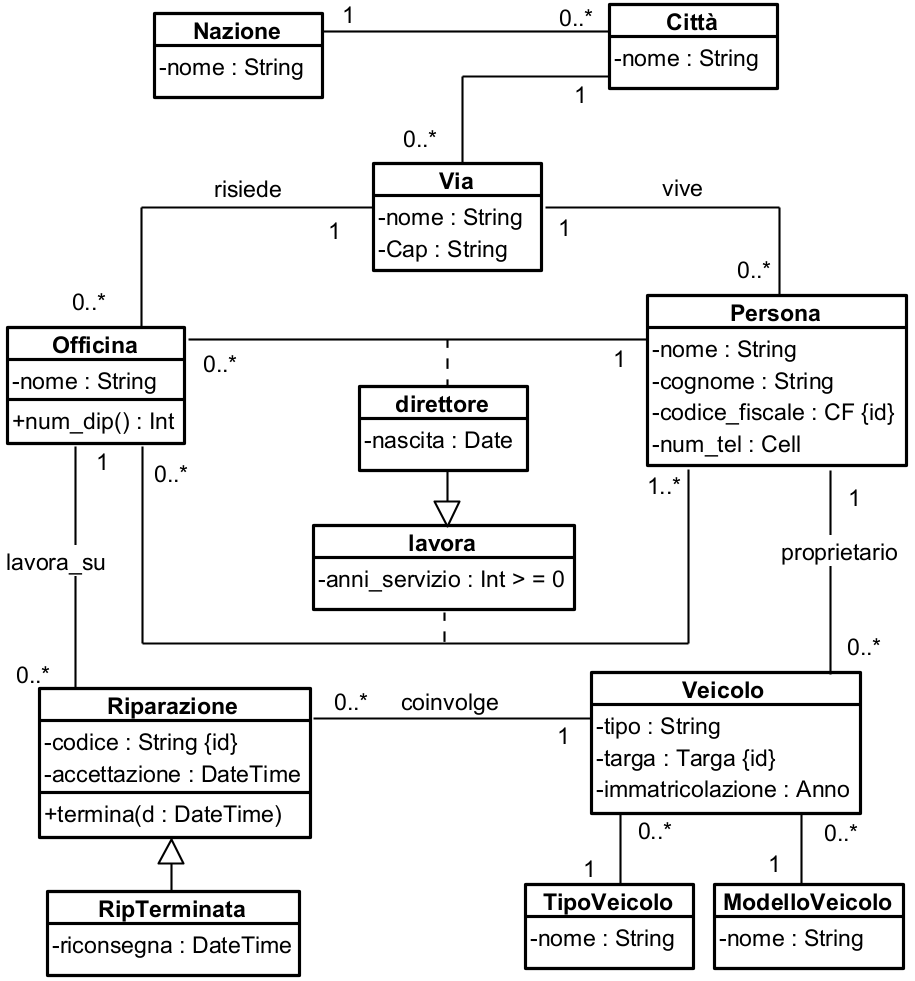
\includegraphics[width=\textwidth]{images/UML.png}
\end{center}
\newpage
\section{Documenti di Specifica}
\subsection{Tipi di Dato}
CF = [A-Z]\{6\} [0-9]\{2\} [A-Z]\{1\} [0-9]\{2\} [A-Z]\{1\} [0-9]\{3\} [A-Z]\{1\}\acc 
Cell = Un codice composto da 10 cifre decimali\acc 
Anno = \{"19" $\lor$ "20"\} concat ["00","99"]\acc 
Targa = Tipo che rispetta l'espressione regolare delle targhe 
\subsection{Specifica delle classi}
\subsubsection{Officina}
Operazione \code{num\_dip() : Int}\begin{itemize}
    \item \textit{pre-condizioni} : L'oggetto di tipo \underline{Officina} che 
    invoca questa operazione, deve essere coinvolto in almeno un link di tipo 
    \underline{lavora} con un oggetto di tipo \underline{Persona}.
    \item \textit{post-condizioni} : Sia $D$ l'insieme dei link di tipo 
    \underline{lavora} in cui è coinvolto l'oggetto invocante, il risultato 
    dell'operazione è $|D|$.
\end{itemize}
\subsubsection{Riparazione}
Operazione \code{termina(d : DateTime)}\begin{itemize}
\item  \textit{pre-condizioni} : L'oggetto di tipo \underline{Riparazione} che invoca 
tale operazione non deve essere anche di tipo \underline{RipTerminata}

\item \textit{post-condizioni} : Sia $r_1=(o,this)$ il link di tipo \underline{lavora\_su}
nella quale è coinvolto l'oggetto invocante, in cui $o$ è un oggetto di tipo \underline{Officina}, 
e sia $r_2=(v,this)$ il link di tipo \underline{coinvolge}
nella quale è coinvolto l'oggetto invocante, in cui $v$ è un oggetto di tipo \underline{Veicolo}.\\

Viene creato un oggetto $T$ di tipo \underline{RipTerminata}, per cui $T.codice=this.codice$ e 
$T.accettazione=this.accettazione$, inoltre $T.riconsegna=d$, si ricordi che $d$ è il parametro 
dell'operazione.\\

Vengono creati i seguenti link $r_1'=(o,T)$, $r_2'=(v,T)$, rispettivamente di tipo \underline{lavora\_su} 
e \underline{coinvolge}. Viene \textit{eliminato} l'oggetto invocante.

\end{itemize}




\end{document}

